\documentclass[aspectratio=169,10pt]{beamer}

% Modern theme
\usetheme{metropolis}
\usepackage{booktabs}
\usepackage{listings}
\usepackage{xcolor}
\usepackage{tikz}
\usetikzlibrary{arrows.meta,positioning,shapes.geometric}

% Colors
\definecolor{tezosblue}{HTML}{2A85A8}
\definecolor{evmpurple}{HTML}{7C3AED}
\definecolor{safegreen}{HTML}{059669}
\definecolor{asmred}{HTML}{DC2626}
\definecolor{codebg}{HTML}{F1F5F9}

\setbeamercolor{progress bar}{fg=tezosblue}
\setbeamercolor{title separator}{fg=tezosblue}
\setbeamercolor{frametitle}{bg=tezosblue!10, fg=black}

\lstset{
  basicstyle=\ttfamily\scriptsize,
  backgroundcolor=\color{codebg},
  frame=none,
  breaklines=true,
  columns=fullflexible,
  keepspaces=true,
  tabsize=2,
}

\lstdefinelanguage{Solidity}{
  keywords={function,returns,return,internal,external,pure,memory,bytes,uint256,int256,bool,string,library,revert,if,else,calldata},
  keywordstyle=\color{evmpurple}\bfseries,
  commentstyle=\color{gray}\itshape,
  morecomment=[l]{//},
}

\title{MichelinePack}
\subtitle{A Verified Michelson PACK Codec for Solidity\\[0.3em]\small\textcolor{gray}{Work in Progress -- Feedback Welcome}}
\author{Paul Laforgue -- Nomadic Labs}
\date{April 8, 2026}
\institute{Core Layer 2}

\begin{document}

% ============================================================
\begin{frame}
\maketitle
\end{frame}

% ============================================================
\begin{frame}{The Problem}

\begin{columns}[T]
\begin{column}{0.45\textwidth}
\textbf{Tezos X} has two runtimes:

\bigskip

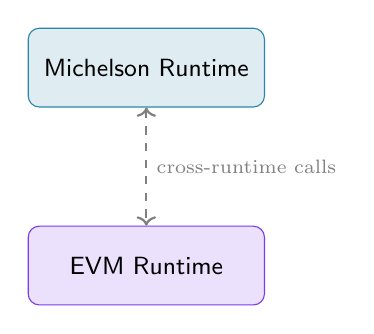
\begin{tikzpicture}[
  box/.style={rectangle, draw, rounded corners=4pt, minimum width=3cm,
    minimum height=1cm, font=\small\sffamily, text centered},
]
  \node[box, fill=tezosblue!15, draw=tezosblue] (mic) {Michelson Runtime};
  \node[box, fill=evmpurple!15, draw=evmpurple, below=1.5cm of mic] (evm) {EVM Runtime};
  \draw[<->, thick, gray, dashed] (mic) -- node[right, font=\scriptsize, text=gray] {cross-runtime calls} (evm);
\end{tikzpicture}
\end{column}

\begin{column}{0.5\textwidth}
Solidity contracts on the EVM side need to \textbf{encode and decode} values
in Michelson's binary \texttt{PACK} format to perform cross-runtime calls
with data payload.

\bigskip

Incorrect serialization can cause \textbf{silent data corruption}, failed
cross-runtime calls, or---in the worst case---\textbf{exploitable vulnerabilities}.

\bigskip

Because this codec sits at the \textbf{trust boundary} between two runtimes,
correctness is critical.
\end{column}
\end{columns}
\end{frame}

% ============================================================
\begin{frame}{The Solution: MichelinePack}

A Solidity library for encoding/decoding \textbf{all 20 packable Michelson types},
backed by \textbf{formal verification}.

\bigskip

\begin{center}
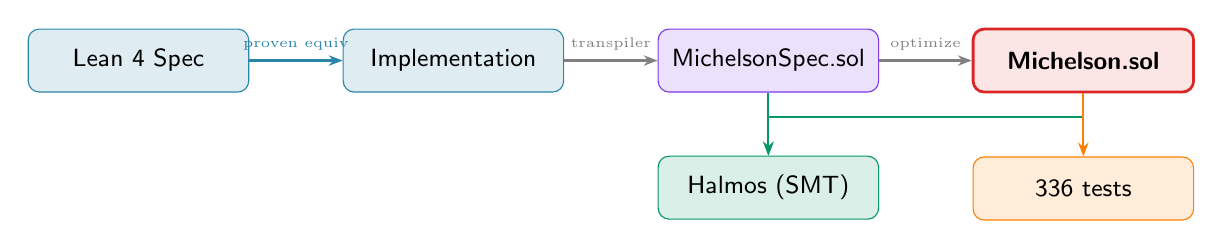
\begin{tikzpicture}[
  every node/.style={font=\small\sffamily},
  box/.style={rectangle, draw, rounded corners=4pt, minimum height=0.8cm,
    minimum width=2.8cm, text centered},
  >={Stealth[length=5pt]},
]
  \node[box, fill=tezosblue!15, draw=tezosblue] (lean) at (0,0) {Lean 4 Spec};
  \node[box, fill=tezosblue!15, draw=tezosblue] (impl) at (4,0) {Implementation};
  \node[box, fill=evmpurple!15, draw=evmpurple] (sol) at (8,0) {MichelsonSpec.sol};
  \node[box, fill=asmred!12, draw=asmred, line width=1pt] (asm) at (12,0) {\textbf{Michelson.sol}};

  \draw[->, thick, tezosblue] (lean) -- node[above, font=\tiny] {proven equiv} (impl);
  \draw[->, thick, gray] (impl) -- node[above, font=\tiny] {transpiler} (sol);
  \draw[->, thick, gray] (sol) -- node[above, font=\tiny] {optimize} (asm);

  \node[box, fill=safegreen!15, draw=safegreen, below=0.8cm of sol] (halmos) {Halmos (SMT)};
  \node[box, fill=orange!15, draw=orange, below=0.8cm of asm] (tests) {336 tests};

  \draw[->, thick, safegreen] (sol) -- (halmos);
  \draw[->, thick, safegreen] (asm.south) -- ++(0,-0.3) -| (halmos);
  \draw[->, thick, orange] (asm) -- (tests);
\end{tikzpicture}
\end{center}

\smallskip
\begin{exampleblock}{Proven roundtrip for all 20 types (e.g.\ \texttt{nat})}
$\forall\, n.\; \texttt{decode}(\texttt{encode}(n)) = n$ \quad\emph{and}\quad
$\forall\, bs,\, n.\; \texttt{decode}(bs) = n \Rightarrow \texttt{encode}(n) = bs$
\end{exampleblock}
\end{frame}

% ============================================================
\begin{frame}[fragile]{API: Encode and Decode}

\begin{lstlisting}[language=Solidity]
// Encode a nat
bytes memory packed = Michelson.pack(Michelson.nat(42));

// Decode a nat
uint256 value = Michelson.toNat(Michelson.unpack(packed));

// Encode a pair of (nat, string)
bytes memory pairPacked = Michelson.pack(
    Michelson.pair(
        Michelson.nat(42),
        Michelson.string_("hello")
    )
);

// Decode a pair
(bytes memory first, bytes memory second) = Michelson.toPair(
    Michelson.unpack(pairPacked)
);
uint256 n = Michelson.toNat(first);
string memory s = Michelson.toString(second);
\end{lstlisting}

\smallskip
\textbf{Rule:} \texttt{pack()} only at the top level. Inner encoders are composable.
\end{frame}

% ============================================================
\begin{frame}[fragile]{Real-World Example: FA2 \texttt{balance\_of}}

\begin{lstlisting}[language=Solidity]
function queryBalance(bytes memory owner, uint256 tokenId) external {
    // Encode params: list(pair(address, nat))
    bytes[] memory requests = new bytes[](1);
    requests[0] = Michelson.pair(
        Michelson.address_(owner), Michelson.nat(tokenId));
    bytes memory params = Michelson.pack(Michelson.list(requests));
    // Cross-runtime call
    (bool success, bytes memory data) = RUNTIME_GATEWAY.call(
        abi.encodeWithSignature("callMichelson(string,string,bytes)",
            "KT1HTYmm7R45F9zY4UcHE7PxpLcCchrjjxYt",
            "balance_of", params));
    // Decode response: list(pair(pair(address, nat), nat))
    bytes[] memory responses = Michelson.toList(Michelson.unpack(data));
    (, bytes memory balBytes) = Michelson.toPair(responses[0]);
    uint256 balance = Michelson.toNat(balBytes);
}
\end{lstlisting}
\end{frame}

% ============================================================
\begin{frame}{20 Supported Types}

\begin{center}
\scriptsize
\begin{tabular}{@{}llll@{}}
\toprule
\textbf{Michelson} & \textbf{Solidity encode} & \textbf{Solidity decode} & \textbf{EVM type} \\
\midrule
\texttt{nat}       & \texttt{nat(n)}          & \texttt{toNat(data)}     & \texttt{uint256} \\
\texttt{int}       & \texttt{int\_(v)}        & \texttt{toInt(data)}     & \texttt{int256} \\
\texttt{bool}      & \texttt{bool\_(b)}       & \texttt{toBool(data)}    & \texttt{bool} \\
\texttt{unit}      & \texttt{unit\_()}         & \texttt{toUnit(data)}    & --- \\
\texttt{string}    & \texttt{string\_(s)}     & \texttt{toString(data)}  & \texttt{string} \\
\texttt{bytes}     & \texttt{bytes\_(d)}      & \texttt{toBytes(data)}   & \texttt{bytes} \\
\texttt{mutez}     & \texttt{nat(uint256(v))} & \texttt{toMutez(data)}   & \texttt{uint64} \\
\texttt{timestamp} & \texttt{int\_(int256(v))} & \texttt{toTimestamp(data)} & \texttt{int64} \\
\midrule
\texttt{pair}      & \texttt{pair(a, b)}      & \texttt{toPair(data)}    & \texttt{(bytes,bytes)} \\
\texttt{or}        & \texttt{left(a)/right(b)} & \texttt{toOr(data)}     & \texttt{(bool,bytes)} \\
\texttt{option}    & \texttt{some(a)/none()}  & \texttt{toOption(data)}  & \texttt{(bool,bytes)} \\
\texttt{list}      & \texttt{list(items)}     & \texttt{toList(data)} & \texttt{bytes[]} \\
\midrule
\texttt{address}   & \texttt{address\_(a)}    & \texttt{toAddress(data)} & \texttt{bytes} (22B) \\
\texttt{key\_hash} & \texttt{keyHash(kh)}     & \texttt{toKeyHash(data)} & \texttt{bytes} (21B) \\
\texttt{signature} & \texttt{signature\_(s)}  & \texttt{toSignature(data)} & \texttt{bytes} \\
\texttt{chain\_id} & \texttt{chainId(id)}     & \texttt{toChainId(data)} & \texttt{bytes4} \\
\bottomrule
\end{tabular}
\end{center}

\smallskip
\centering + \texttt{map}, \texttt{set}, \texttt{key}, \texttt{contract} (20 total)
\end{frame}

% ============================================================
\begin{frame}{Safety: What Happens on Bad Input?}

Every error case \textbf{reverts} with a specific, descriptive error:

\bigskip

\begin{center}
\begin{tabular}{@{}ll@{}}
\toprule
\textbf{Condition} & \textbf{Solidity error} \\
\midrule
Value too large for \texttt{uint256} & \texttt{revert IntOverflow()} \\
Negative value in nat decoder       & \texttt{revert NatNegative()} \\
Truncated input                     & \texttt{revert InputTruncated()} \\
Wrong Micheline node tag             & \texttt{revert UnexpectedNodeTag(expected, got)} \\
Non-canonical encoding              & \texttt{revert TrailingZeroByte()} \\
Negative zero (\texttt{0x40})       & \texttt{revert NegativeZero()} \\
\bottomrule
\end{tabular}
\end{center}

\bigskip
\textbf{No silent truncation. No undefined behavior.} If decoding fails, the transaction reverts cleanly.
\end{frame}

% ============================================================
\begin{frame}{Gas Performance: Assembly Optimization}

The library ships two implementations:

\begin{itemize}
  \item \textbf{MichelsonSpec.sol} --- reference (transpiled from verified spec)
  \item \textbf{Michelson.sol} --- production (hand-optimized assembly)
\end{itemize}

\bigskip

\begin{center}
\begin{tabular}{@{}lrrrr@{}}
\toprule
\textbf{Operation} & \textbf{Spec} & \textbf{Assembly} & \textbf{Savings} \\
\midrule
\texttt{packNat(42)}            & 821     & 120     & 85\% \\
\texttt{packNat(uint256.max)}   & 17,961  & 3,316   & 82\% \\
\texttt{unpackNat(42)}          & 1,546   & 263     & 83\% \\
\texttt{unpackInt(int256.min)}  & 32,330  & 6,781   & 79\% \\
\texttt{unpackBool}             & 1,432   & 217     & 85\% \\
\texttt{unpackString(256B)}     & 135,881 & 1,048   & \textbf{99\%} \\
\bottomrule
\end{tabular}
\end{center}

\smallskip
\centering\textbf{79--99\% gas savings} on atom operations. Composites delegate to spec.
\end{frame}

% ============================================================
\begin{frame}{How Do We Know the Assembly Is Correct?}

\textbf{Halmos} --- symbolic execution with SMT solver (Z3).

\bigskip

Not testing with random values. \textbf{Proving for ALL possible inputs}:

\begin{itemize}
  \item \texttt{asm\_decode(x) == spec\_decode(x)} for every \texttt{uint256}/\texttt{int256}
  \item \texttt{asm\_rejects(bytes) $\Leftrightarrow$ spec\_rejects(bytes)} for arbitrary byte sequences
  \item \texttt{unpack(pack(x)) == x} on actual compiled bytecode
\end{itemize}

\bigskip

\begin{center}
\textbf{40 symbolic checks}, all passing.\\
Including adversarial checks: 7,011 symbolic paths for int, 3,511 for nat.
\end{center}

\bigskip
\begin{exampleblock}{Key insight}
Halmos verifies the \emph{compiled bytecode}, not the source code.\\
Even compiler bugs would be caught.
\end{exampleblock}
\end{frame}

% ============================================================
\begin{frame}{Test Coverage: Four Layers}

\begin{center}
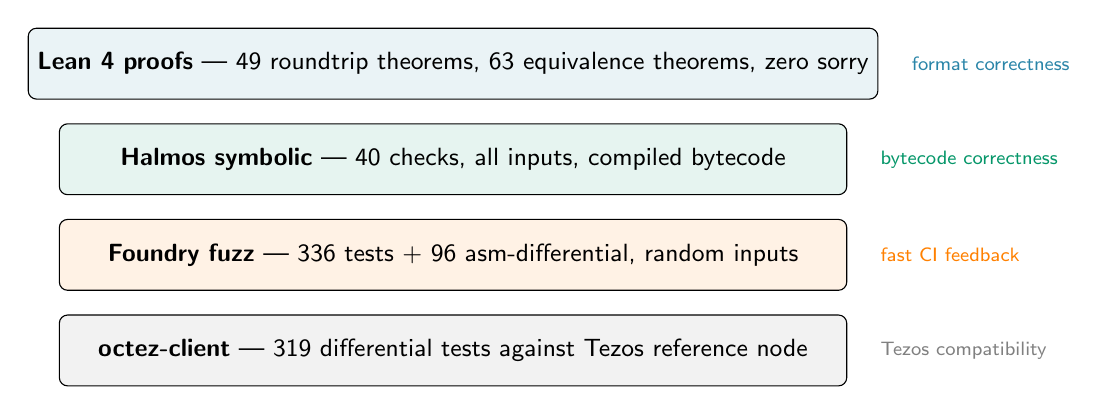
\begin{tikzpicture}[
  layer/.style={rectangle, draw, rounded corners=3pt, minimum width=10cm,
    minimum height=0.9cm, font=\small\sffamily, text centered},
]
  \node[layer, fill=tezosblue!10] (l1) at (0,0)
    {\textbf{Lean 4 proofs} --- 49 roundtrip theorems, 63 equivalence theorems, zero sorry};
  \node[layer, fill=safegreen!10, below=0.3cm of l1] (l2)
    {\textbf{Halmos symbolic} --- 40 checks, all inputs, compiled bytecode};
  \node[layer, fill=orange!10, below=0.3cm of l2] (l3)
    {\textbf{Foundry fuzz} --- 336 tests + 96 asm-differential, random inputs};
  \node[layer, fill=gray!10, below=0.3cm of l3] (l4)
    {\textbf{octez-client} --- 319 differential tests against Tezos reference node};

  \node[right=0.3cm of l1, font=\scriptsize\sffamily, text=tezosblue] {format correctness};
  \node[right=0.3cm of l2, font=\scriptsize\sffamily, text=safegreen] {bytecode correctness};
  \node[right=0.3cm of l3, font=\scriptsize\sffamily, text=orange] {fast CI feedback};
  \node[right=0.3cm of l4, font=\scriptsize\sffamily, text=gray] {Tezos compatibility};
\end{tikzpicture}
\end{center}

\bigskip
\centering \textbf{$\sim$900 total checks} across all layers.
\end{frame}

% ============================================================
\begin{frame}{The Verified Pipeline}

Every step is connected --- no manual translation gaps:

\bigskip

\begin{center}
\small
\textcolor{tezosblue}{\fbox{Lean 4 Spec}}
$\xrightarrow{\text{\tiny 63 proofs}}$
\textcolor{tezosblue}{\fbox{Implementation}}
$\xrightarrow{\text{\tiny transpiler}}$
\textcolor{evmpurple}{\fbox{MichelsonSpec.sol}}
$\xrightarrow{\text{\tiny derive}}$
\textcolor{asmred}{\fbox{\textbf{Michelson.sol}}}

\medskip
\scriptsize
\textcolor{tezosblue}{49 roundtrip theorems} \quad
\textcolor{tezosblue}{zero sorry} \quad
\textcolor{evmpurple}{53 functions from IR} \quad
\textcolor{asmred}{79--99\% gas savings}
\end{center}

\bigskip

\begin{itemize}
  \item Byte validity enforced by \textbf{types} (\texttt{Fin 256}) --- not proof obligations
  \item Both roundtrips proven for \textbf{all 20 types}: no information loss \emph{and} canonical uniqueness
  \item All 52 Solidity functions generated from structured IR --- no hand-written template strings
\end{itemize}
\end{frame}

% ============================================================
\begin{frame}{Compatibility with Tezos}

\textbf{319 differential tests} against \texttt{octez-client} (the Tezos reference implementation):

\bigskip

\begin{itemize}
  \item Our output compared \textbf{directly} against \texttt{octez-client} output --- no hardcoded expected values
  \item Covers all 20 types including nested composites
  \item Boundary values at every zarith byte transition ($2^6$, $2^{13}$, $2^{20}$, \ldots)
  \item Cross-type consistency checks: \texttt{nat(42) == int(42)}, \texttt{nat(v) == mutez(v)}
  \item Nested composites: 4-deep pairs, lists of options, maps with string keys
\end{itemize}

\bigskip
\begin{center}
\textbf{Every value we encode matches what Tezos produces.}
\end{center}
\end{frame}

% ============================================================
\begin{frame}{What Properties Are Guaranteed?}

\begin{center}
\renewcommand{\arraystretch}{1.3}
\begin{tabular}{@{}lll@{}}
\toprule
\textbf{Property} & \textbf{What it means} & \textbf{How it's verified} \\
\midrule
$\texttt{decode}(\texttt{encode}(x)) = x$ & No information loss & Lean proof \\
$\texttt{decode}(bs) = x \Rightarrow \texttt{encode}(x) = bs$ & Unique encoding & Lean proof \\
\texttt{asm(x) == spec(x)} & Assembly is faithful & Halmos (all inputs) \\
\texttt{our\_output == octez\_output} & Tezos compatible & 319 diff tests \\
Bad input $\to$ revert & No silent failures & 10 typed errors \\
Bytes $< 256$ & Valid byte range & \texttt{Fin 256} type \\
\bottomrule
\end{tabular}
\end{center}

\bigskip
\begin{center}
\textbf{Zero sorry} (unproven assumptions) in the entire Lean codebase.\\
\textbf{Zero axioms.} \textbf{Zero partial functions.}
\end{center}
\end{frame}

% ============================================================
\begin{frame}{Summary}

\begin{columns}[T]
\begin{column}{0.5\textwidth}
\textbf{For developers:}
\begin{itemize}
  \item Clean API: \texttt{pack(nat(42))}
  \item 20 Michelson types
  \item Descriptive error messages
  \item 79--99\% gas savings with assembly
  \item Drop-in Solidity library
\end{itemize}
\end{column}

\begin{column}{0.45\textwidth}
\textbf{For security:}
\begin{itemize}
  \item Machine-checked proofs (Lean 4)
  \item Bytecode-level verification (Halmos)
  \item 319 octez-client diff tests
  \item 336 Foundry fuzz tests
  \item Both roundtrips for all types
\end{itemize}
\end{column}
\end{columns}

\bigskip
\begin{center}
\large
\textbf{Safe cross-runtime calls on Tezos X.}
\end{center}
\end{frame}

% ============================================================
\begin{frame}{Status \& Next Steps}

This project is a \textbf{work in progress}. We are looking for feedback on:

\bigskip

\begin{itemize}
  \item \textbf{API design} --- is it intuitive for Solidity developers?
  \item \textbf{Type coverage} --- are there missing types you need?
  \item \textbf{Integration} --- how would you use this in a real cross-runtime dApp?
  \item \textbf{Packaging} --- Foundry package? npm wrapper? SDK?
\end{itemize}

\bigskip

\textbf{What's next:}
\begin{itemize}
  \item Documentation
  \item End-to-end cross-runtime test on Tezos X testnet
  \item CI pipeline with automated verification
  \item Package distribution (Foundry registry)
\end{itemize}

\bigskip
\centering
\large\textbf{Questions? Feedback?}\\[0.3em]
\normalsize\texttt{github.com/phink/tx-codec}
\end{frame}

\end{document}
